\chapter{Wien bridge oscillator and digital electronic}
In the first part of the experience we built a wien bridge oscillator with an automatic gain control (AGC) which was made possibile by the variable resistance of a tungsten light bulb. We analized the wave's quality and the critical startup time. The second part was about digital electronics: after some exercise with some NAND ports we designed a circuit for an hypotetical rough house alarm system.

\section{Materials}
\begin{itemize}
\item Resistors, trimmers, capacitors
\item A tungsten light bulb
\item Power supply RIGOL DP831A
\item Waveform generator RIGOL DG1032
\item Multimeter RIGOL DM3068
\item uA741
\item 8-bit LED viewer
\item DM74LS00
\end{itemize}
The resistors and capacitors used were all with an uncertainty of 5\% of their nominal value

\section{Experimental setup}

\subsection{Wien brigde oscillator}
Regarding the band-pass filter in the positive feedback branch, we used two resistors and two capacitors identical in pairs ($R = 10.0 \pm 0.5 k\Omega, C = 15.0 \pm 0.7 nF$): that way we had a passing frequency of $1060 \pm 70$ Hz, attenuated by a factor $\frac{1}{3}$. 
In order to make the wien bridge stably oscillating we then needed a gain factor G of 3 from our op-amp, that means we had to choose $R_2 = 2 R_1$: for a better precision we used a $1 k\Omega$ trimmer as $R_2$ and as $R_1$ a resistor of $47.0 \pm 2.3 \Omega$ subsequently followed by a PTC (positive temperature coefficient) tungsten light with a resistance depending on its own temperature.\\
We set the trimmer to a resistance a little lower than twice 47 $\Omega$, in order to adjust it carefully: once powered the circuit in fact, we raised slowly the trimmer resistance till the output switched from continous 0 V to an oscillating (but unstable) signal.\\
At this point we placed the light bulb after the 47 $\Omega$ resistor: Turning on the circuit, the current would then start to flow in the tungsten resistor increasing its resistance (thanks to the heat produced by the current), bringing the total one ($R_1$) till the exact half value of the trimmer one thanks to the thermal inertia.\\
Our circuit would now auto-oscillate stably, but however the process would have required some time after the power on to equilibrate.
\begin{figure}[H]
\centering
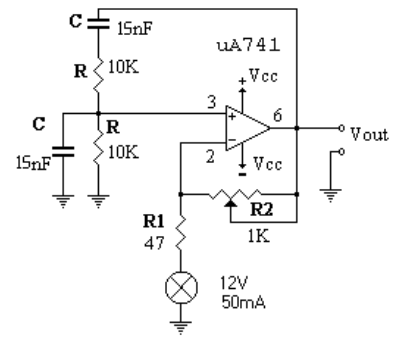
\includegraphics[width=.7\textwidth]{9/wien.png}
\caption{Wien bridge}\label{wien}
\end{figure}

\subsection{Logic gates}
We needed to work with some DM74LS00 components, so firstly we tested them in a NAND configuration with the help of the 8-bit LED viewer for a visual confirmation.
For designing the alarm system logic circuit we wrote the desired table of true with which we built the Karnaugh map (table 8.1) and we minimized it.

\begin{table}[H]
\centering
\label{my-label}
\begin{tabular}{lllll}
\hline
 DW/IK & 00 & 01 & 11 & 10 \\ \hline
 00    & 0  & 0  & 0  & 1 \\
 01    & 1  & 1  & 1  & 1 \\
 11    & 1  & 1  & 1  & 1 \\ 
 10    & 1  & 1  & 1  & 1 \\ \hline
\end{tabular}\caption{D = Door, W = Window, I = Infrared, K = Key}
\end{table}
The simplified form found was $Y = D + W + I\overline{K}$. The problem was that we only had NAND gates so we needed to write AND, OR and NOT with NAND: this is how to do it
\begin{itemize}
\item NOT is the easiest one, because you only need to connect the signal you want to negate in both NAND inputs
\item AND at this point is easy too: it just needs a negation after a simple NAND
\item OR is made by negating the inputs of a NAND
\end{itemize}

\section{Data analysis}
In figure \ref{starting} we can see that the output has a transitorial stage that lasts nearly 7.5 s before stabilizing and forming a sine wave (see figure \ref{stable}) of frequency $f_{exp} = 1122.1 \pm 1.4$ Hz: this frequency is actually compatible with the theoretical attended value, $f_{theo} = 1060 \pm 70$ Hz.
\begin{figure}[H]
\centering
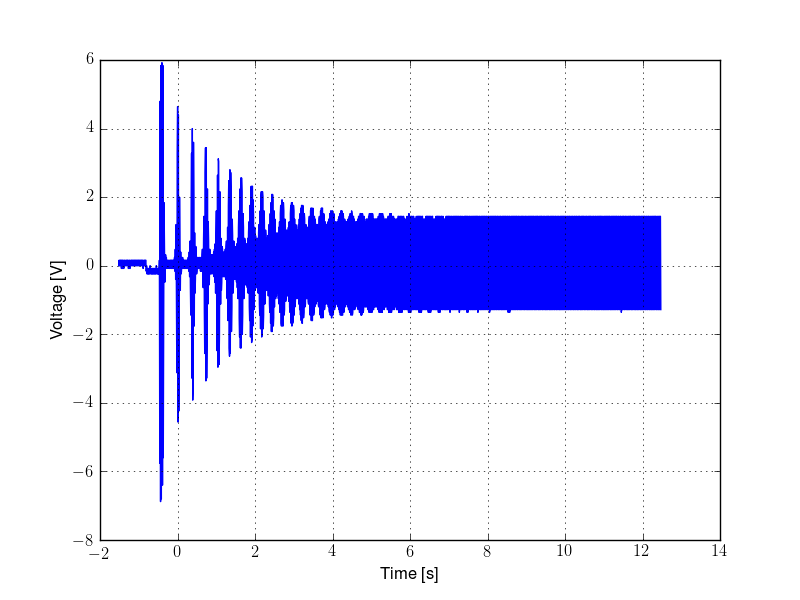
\includegraphics[width=.7\textwidth]{9/starting.png}
\caption{Starting process of the wien bridge}\label{starting}
\end{figure}
\begin{figure}[H]
\centering
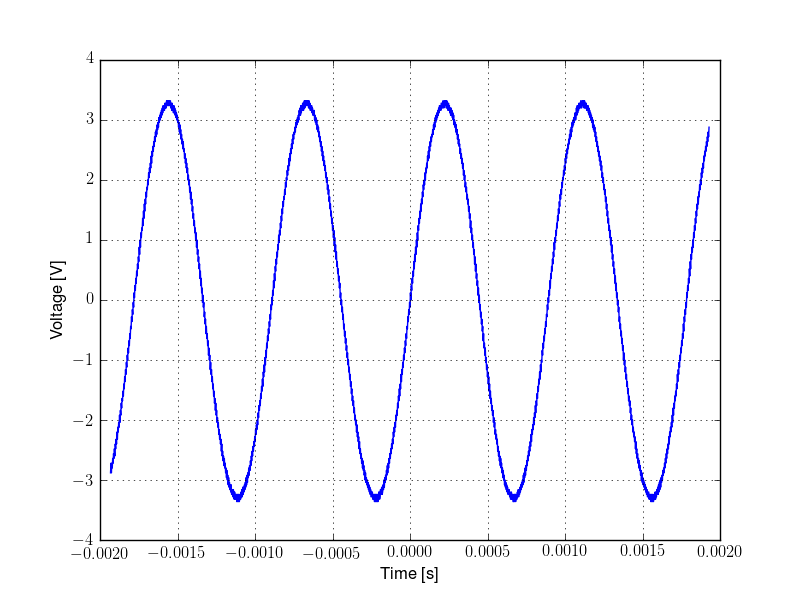
\includegraphics[width=.7\textwidth]{9/stable.png}
\caption{Stable state of the wien bridge}\label{stable}
\end{figure}
We also tested the circuit removing the by-pass capacitors but, as we can see in figure \ref{without_bypass}, the noise is too high for allowing a stable state.
\begin{figure}[H]
\centering
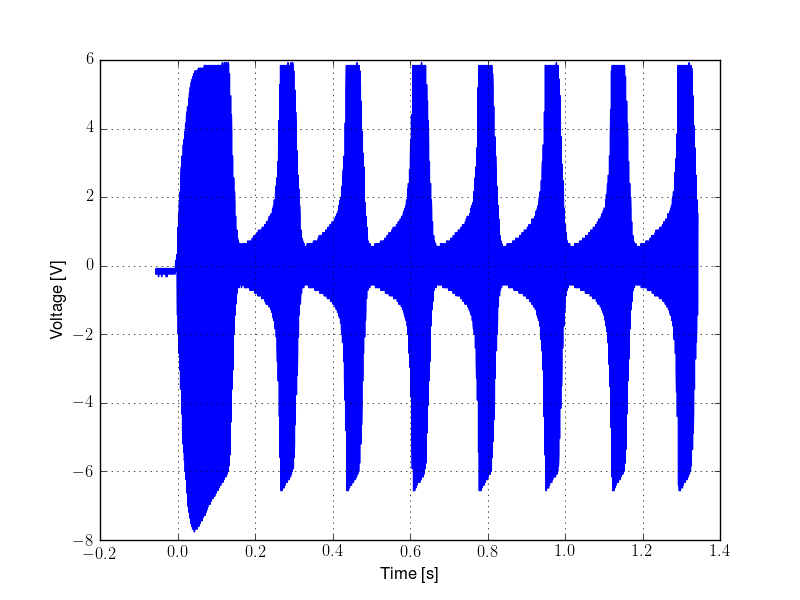
\includegraphics[width=.7\textwidth]{9/without_bypass.png}
\caption{Bridge without the by-pass capacitors}\label{without_bypass}
\end{figure}
